\documentclass[12pt]{article}
\usepackage[a4paper, left=3cm, right=3cm, top=3.5cm, bottom=3.5cm]{geometry}
\usepackage{graphicx} % Required for inserting images
\usepackage{amsmath}
\usepackage{amsthm}
\usepackage{amssymb}
\usepackage{xcolor}
\usepackage{hyperref} % pour des liens cliquables dans le PDF
\usepackage[english]{babel} % pour la langue anglaise
\usepackage{titling} % pour personnaliser le titre

\renewcommand{\proofname}{Demonstration :}

% Informations de l'encadré et du titre
\title{\huge\textbf{Academic Research Project :  Gaussian correlation inequality}}
\author{
    \textbf{Tom De Oliveira}\\
    \textbf{Victor Kerlou}
}
\date{June 2025}

% Personnalisation du titre
\pretitle{\begin{center}\huge\bfseries}
\posttitle{\end{center}}
\preauthor{\begin{center}\Large}
\postauthor{\end{center}}
\predate{\begin{center}\large}
\postdate{\end{center}}

\begin{document}

% Page de titre
\maketitle

\vspace{1cm} % Un peu d'espace pour aérer

% Insertion de la photo (illustration du sujet ou de l'approche mathématique)
\begin{center}
    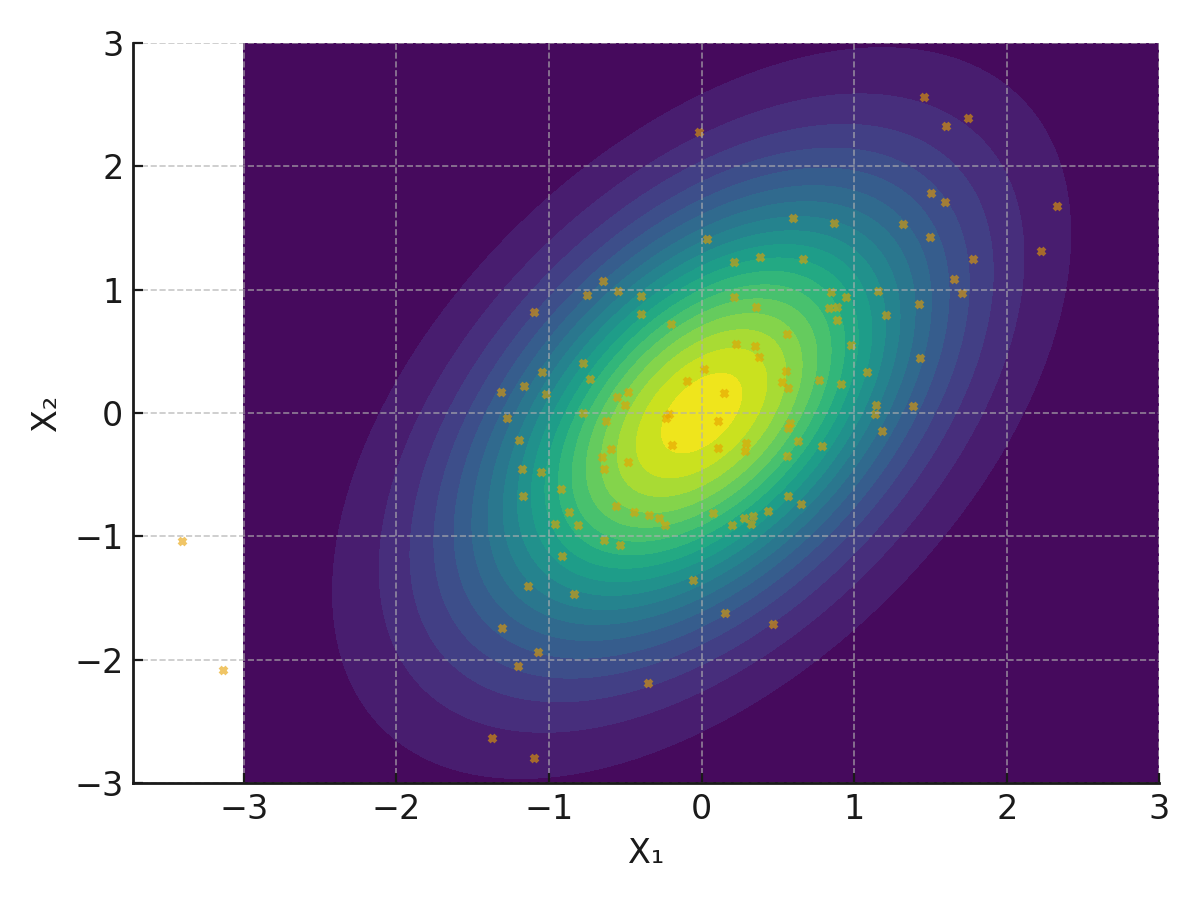
\includegraphics[width=0.35\textwidth]{photo.png} \\[1em]
    \textit{Illustration: Gaussian distribution darts}
\end{center}

\vspace{2cm} % Un peu d'espace avant le texte principal

% Encadré du sujet et de l'encadrant
\begin{flushright}
    \textbf{Supervised by :} \\
    \textit{Paul Dario}
\end{flushright}

\vspace{1cm} % Un peu d'espace après l'encadré

\newpage % Crée une nouvelle page pour le début du contenu

\begin{abstract}
The first section on the introduction to Gaussian vectors was inspired by the aggregation preparation course by Jean-Jacques Ruch \cite{ruch}.
The second and third sections were inspired by a 2018 thesis from ENS Paris by Houcine Ben Dali and Severin Benzoni \cite{benzoni}, as well as by Franck Barthe's summary of the proof in the Bourbaki seminar \cite{barthe}. The last two references \cite{Royen} and \cite{Matlak} correspond to the original proof and its reformulation.
\end{abstract}

\newpage
\renewcommand{\contentsname}{Summary}
\tableofcontents % Génère automatiquement le sommaire

\newpage

\section{Introduction to Gaussian Vectors}

Gaussian vectors are the natural generalization in $d$ dimensions of one-dimensional Gaussian random variables. Throughout this work, we consider a probability space $(\Omega, \mathcal{F}, \mathbb{P})$.

\vspace{0.3cm}

\textbf{Definition 1.1.}

Let $\mathbf{X}$ be a random (column) vector in $\mathbb{R}^d$ whose components are square-integrable. The mean vector of $\mathbf{X}$ is as follows:

\[
\mathbb{E}(\mathbf{X}) =
\begin{pmatrix}
\mathbb{E}(X_1) \\
\vdots \\
\mathbb{E}(X_d)
\end{pmatrix}
\]
and its covariance matrix is given by :
\[
\mathrm{Var}(\mathbf{X}) = \mathbb{E}\!\left[(\mathbf{X} - \mathbb{E}[\mathbf{X}])(\mathbf{X} - \mathbb{E}[\mathbf{X}])^\top\right] =
\begin{pmatrix}
\mathrm{Var}(X_1) & \mathrm{Cov}(X_1, X_2) & \cdots & \mathrm{Cov}(X_1, X_d) \\
\mathrm{Cov}(X_2, X_1) & \mathrm{Var}(X_2) & \cdots & \mathrm{Cov}(X_2, X_d) \\
\vdots & \vdots & \ddots & \vdots \\
\mathrm{Cov}(X_d, X_1) & \mathrm{Cov}(X_d, X_2) & \cdots & \mathrm{Var}(X_d)
\end{pmatrix}
\]

\textbf{Theorem 1.1.}\\
The covariance matrix is a symmetric positive semi-definite matrix.

\begin{proof}
The symmetry of the covariance matrix is evident by construction. Recall that a matrix is positive semi-definite if and only if, for every vector $\mathbf{v} \in \mathbb{R}^d$, we have
\[
\mathbf{v}^\top A \mathbf{v} \geq 0.
\]
Let $\mathbf{v} \in \mathbb{R}^d$, we want to show that
\[
\mathbf{v}^\top \mathrm{Var}(\mathbf{X}) \mathbf{v} \geq 0.
\]
We begin by expanding the expression of the variance:
\[
\mathbf{v}^\top \mathrm{Var}(\mathbf{X}) \mathbf{v} = \mathbb{E}\!\left[\mathbf{v}^\top (\mathbf{X} - \mathbb{E}[\mathbf{X}]) (\mathbf{X} - \mathbb{E}[\mathbf{X}])^\top \mathbf{v}\right].
\]
We see that
\[
\mathbf{v}^\top (\mathbf{X} - \mathbb{E}[\mathbf{X}]) (\mathbf{X} - \mathbb{E}[\mathbf{X}])^\top \mathbf{v} = \left( \mathbf{v}^\top (\mathbf{X} - \mathbb{E}[\mathbf{X}]) \right)^2.
\]
Therefore, by the positivity of the expectation
\[
\mathbb{E}\!\left[\left( \mathbf{v}^\top (\mathbf{X} - \mathbb{E}[\mathbf{X}]) \right)^2\right] \geq 0.
\]
Hence
\[
\mathbf{v}^\top \mathrm{Var}(\mathbf{X}) \mathbf{v} \geq 0.
\]
\end{proof}

\newpage

\textbf{Definition 1.2.}
A random variable $\mathbf{X} = (X_1, \dots, X_n) \in \mathbb{R}^n$ is called a Gaussian vector if for every $\mathbf{a} = (a_1, \dots, a_n) \in \mathbb{R}^n$, the real-valued random variable $\langle \mathbf{a}, \mathbf{X} \rangle = a_1 X_1 + \dots + a_n X_n$ is Gaussian.

\vspace{0.3cm}

We therefore observe that if $X$ is Gaussian, each of its components is also Gaussian since the mapping
\[
(X_1, X_2, \ldots, X_d) \mapsto X_i
\]
is a linear form.
However, the converse is not true in general!

\vspace{0.3cm}

\textbf{Theorem 1.2.} Let $X$ be a random vector in $\mathbb{R}^d$. The following statements are equivalent:
\begin{enumerate}
    \item The vector $X$ is Gaussian with mean $\mathbf{m}$ and covariance matrix $\Gamma$.
    \item The characteristic function of $X$ is given by: for all $u \in \mathbb{R}^d$,
    \[
    \Phi_X(u) = \mathbb{E}\!\left[ \exp(i u^\top X) \right] = \exp\!\left( i u^\top \mathbf{m} - \frac{1}{2} u^\top \Gamma u \right).
    \]
\end{enumerate}

\begin{proof}
The function $X \mapsto u^\top X$ is linear, so by the definition of a Gaussian vector, $u^\top X$ is Gaussian with mean $\alpha$ and variance $\sigma^2$.\\
We have:
\[
\alpha = \mathbb{E}(u^\top X) = u^\top \mathbb{E}(X)
\]
and
\[
\sigma^2 = \mathrm{Var}(u^\top X) = u^\top \Gamma u.
\]
We know the characteristic function of a univariate Gaussian distribution
\[
\varPhi_{u^\top X}(x) = \exp\!\left(i \alpha x - \frac{\sigma^2 x^2}{2}\right)
= \exp\!\left(i x\, u^\top \mathbb{E}(X) - \frac{x^2}{2} u^\top \Gamma u\right).
\]
Substituting back into the expression for the characteristic function of $X$, we get
\[
\varPhi_X(u) = \exp\!\left(i u^\top m - \frac{1}{2} u^\top \Gamma u\right).
\]
Since the characteristic function uniquely determines the distribution, this concludes the proof.
\end{proof}

\vspace{0.3cm}

\textbf{Theorem 1.3. }
Let $X$ be a Gaussian vector with mean $m$ and covariance matrix $\Gamma$. Let $Z$ be a standard Gaussian vector and $A$ a square root matrix of $\Gamma$. Then the vectors $X$ and $m + AZ$ have the same distribution.

\begin{proof}
Let $X$ be a Gaussian vector with mean $m$ and variance $\Gamma$.
Let $A$ be a matrix such that $A = \sqrt{\Gamma}$,
and let $Z$ be a standard Gaussian vector.
Consider the random variable $m + AZ$.
It is clear that:
\[
\mathbb{E}(m + AZ) = m + \mathbb{E}(AZ) = m \quad \text{since} \quad \mathbb{E}(Z) = 0.
\]
Moreover,
\[
\mathrm{Var}(m + AZ) = \mathrm{Var}(AZ) = A^2 \mathrm{Var}(Z) = \Gamma \quad \text{since} \quad \mathrm{Var}(Z) = I_d.
\]
It remains to show that $m + AZ$ is indeed a Gaussian vector.
Let $\mathbf{a} \in \mathbb{R}^d$,
\[
\mathbf{a}^\top (m + AZ) = \mathbf{a}^\top m + \mathbf{a}^\top (AZ).
\]
Since $Z$ is a Gaussian vector, $AZ$ is also Gaussian because it is the result of a linear transformation.
Therefore, $AZ$ remains a Gaussian vector.
As a result, $m + AZ$ is also a Gaussian vector, and it has the same distribution as $X$.
\end{proof}

\textbf{Theorem 1.4. }\\
For any Gaussian vector $X \in \mathbb{R}^d$, the following properties are equivalent
\begin{enumerate}
    \item The components $X_1, \dots, X_d$ are mutually independent.
    \item The components $X_1, \dots, X_d$ are pairwise independent.
    \item The covariance matrix $\Gamma$ of $X$ is diagonal.
\end{enumerate}

\begin{proof}
The implications $1. \Rightarrow 2. \Rightarrow 3.$ are straightforward. Let us prove $3. \Rightarrow 1.$ \\
If $\Gamma = \mathrm{Diag}(\sigma_1^2, \dots, \sigma_n^2)$, then for any $u \in \mathbb{R}^d$,
\[
\Phi_X(u) = \exp\!\left(i u^\top m - \frac{1}{2} u^\top \Gamma u\right)
= \exp\!\left(i \sum_{j=1}^d u_j m_j - \frac{1}{2} \sum_{j=1}^d \sigma_j^2 u_j^2 \right).
\]
This factors as:
\[
\Phi_X(u) = \prod_{j=1}^d \exp\!\left(i u_j m_j - \frac{1}{2} \sigma_j^2 u_j^2\right)
= \prod_{j=1}^d \Phi_{X_j}(u_j).
\]
\end{proof}

\vspace{0.3cm}

\textbf{Remark:}
In particular, a Gaussian vector has independent components if and only if, for all $i \neq j$, we have
\[
\mathrm{Cov}(X_i, X_j) = 0.
\]
For example, a standard Gaussian vector always has independent components, each following a $\mathcal{N}(0, 1)$ on $\mathbb{R}$.

\vspace{0.3cm}

\textbf{Theorem 1.5.}
The Gaussian distribution $\mathcal{N}(m, \Gamma)$ on $\mathbb{R}^d$ admits a probability density function with respect to the Lebesgue measure on $\mathbb{R}^d$ if and only if $\Gamma$ is invertible.
In that case, the density $f$ is given by:

For all $x \in \mathbb{R}^d$,
\[
f(x) = \frac{1}{\sqrt{(2\pi)^d \det(\Gamma)}} \exp \left( -\frac{1}{2} (x - m)^\top \Gamma^{-1} (x - m) \right).
\]

\begin{proof}
The Gaussian distribution $N(m, \Gamma)$ can be seen as the distribution of the random vector
$m + AZ$, where $Z$ is a Gaussian vector in $\mathbb{R}^d$ with independent components, each following the
$N(0, 1)$ distribution. As a result, the density of $Z$ is
\[
f_Z(z) = \prod_{i=1}^{d} \frac{1}{\sqrt{2\pi}} \exp\left( -\frac{1}{2} z_i^2 \right)
= \frac{1}{\sqrt{(2\pi)^d}} \exp\left( -\frac{1}{2} \|Z\|^2 \right).
\]
If $X \sim N(m, \Gamma)$, then for any bounded continuous function $h : \mathbb{R}^d \to \mathbb{R}$,
\[
\mathbb{E}[h(X)] = \mathbb{E}[h(AZ + m)] = \int_{\mathbb{R}^d} h(Az + m) f_Z(z) \, dz.
\]
The decomposition $\Gamma = A A^\top$ implies that $|\det(A)| = \sqrt{\det(\Gamma)}$. Moreover, $\Gamma$ is invertible if and only if $A$ is invertible, in which case  $\Gamma^{-1} = (A^{-1})^\top A^{-1}$.
Besides, the affine change of variable $x = Az + m$ is a diffeomorphism from $\mathbb{R}^d$ onto itself if and only if $A$ is invertible. Its Jacobian is then equal to $\det(A^{-1})$. It follows that
\[
\mathbb{E}[h(X)] = \frac{1}{\sqrt{(2\pi)^d \det(\Gamma)}} \int_{\mathbb{R}^d} h(x) \exp\left( -\frac{1}{2} (x - m)^\top \Gamma^{-1} (x - m) \right) \, dx,
\]
which explains the stated formula for the density $f$.
\end{proof}

\newpage

\section{Gaussian correlation inequality}

The Gaussian correlation inequality was conjectured in its general form in 1972 and remained open for more than 40 years until it was resolved by Thomas Royen. The proof of this result is the subject of this study.

\subsection{Statement of the conjecture}

Let $X := (X_1, \dots, X_n)$ be a Gaussian vector in $\mathbb{R}^n$ and let $E, F \subseteq \mathbb{R}^n$ be two convex and symmetric sets. Then
\[
\mathbb{P}(X \in E \cap F) \geq \mathbb{P}(X \in E) \mathbb{P}(X \in F).
\]

\subsection{Geometric approach}
The goal of this section is to show that it is sufficient to study the Gaussian correlation on simpler sets, \emph{polyhedra}.

\vspace{0.3cm}
\textbf{Definition 2.1} A polyhedron $A$ in $\mathbb{R}^n$ is a closed convex set that can be written as a finite intersection of half-spaces, that is to say:
\[
A = \bigcap_{i=1}^{n} \left\{ x \in \mathbb{R}^n \mid \langle x, u_i \rangle \leq a_i \right\},
\]
for some vectors $u_i \in \mathbb{R}^n$ and real numbers $(a_i)_{1 \leq i \leq n}$.\\

\vspace{0.3cm}

\textbf{Definition 2.2.} Let $K \subset \mathbb{R}^n$. The \emph{polar} of $K$ is the set:
\[
K^\circ = \left\{ y \in \mathbb{R}^n \mid \langle x, y \rangle \leq 1, \ \forall x \in K \right\}.
\]

\vspace{0.3cm}

\textbf{Theorem 2.1.}
Let $K$ be a non-empty closed symmetric convex set.
Then $K = K^{\circ\circ}$.

\begin{proof}
The first inclusion $K \subseteq K^{\circ\circ}$ follows directly from the definition of the polar set. Let $x \in K$, we want to show that $\langle x, y \rangle \leq 1$ for all $y \in K^\circ$. If $y \in K^\circ$, by definition, then $\langle x, y \rangle \leq 1$, which implies $x \in K^{\circ\circ}$.
For the other inclusion, we suppose that $x_0 \notin K$. Since $K$ is closed, by the Hahn--Banach separation theorem, there exists $y \in \mathbb{R}^n$ and $\alpha \in \mathbb{R}$ such that
\[
\forall x \in K, \quad \langle x, y \rangle < \alpha < \langle x_0, y \rangle.
\]
Since $0 \in K$, we have $\alpha \neq 0$. Dividing by $\alpha$, we may assume that $\alpha = 1$. Hence, $y \in K^{\circ}$ and
\[
\langle y, x_0 \rangle > 1,
\]
which implies $x_0 \notin K^{\circ\circ}$.
\end{proof}

\textbf{Theorem 2.2.} Let $K$ be a symmetric convex set. Then there exists a decreasing sequence of symmetric polyhedra $K_n$ such that
\[
K = \bigcap_{n \in \mathbb{N}} K_n.
\]

\textbf{Remark.} We can always assume the convex sets under study are closed, since
\[
\gamma(K) = \gamma(\overline{K}).
\]

\begin{proof}
Let $(x_n)_{n \geq 0}$ be a sequence of points that is dense in $K^\circ$. We define:
\[
K_n := \bigcap_{0 \leq i \leq n} \{ x \in \mathbb{R}^n \mid |\langle x, x_i \rangle| \leq 1 \}.
\]
It is clear that the sequence of polyhedra $(K_n)_{n \geq 0}$ is decreasing, and that $K^{\circ\circ} \subset K_n$.

But, from the previous theorem, $K = K^{\circ\circ}$, so
\[
K \subset \bigcap_{n \in \mathbb{N}} K_n.
\]
Conversely, if $x \in \bigcap_{n \in \mathbb{N}} K_n$, by the density of $(x_n)_{n \geq 0}$, we have
\[
\forall y \in K^\circ, \quad \langle x, y \rangle \leq 1.
\]
Thus, $x \in K^{\circ\circ} = K$, which concludes the proof.
\end{proof}

\vspace{0.3cm}

It is therefore sufficient to prove the Gaussian correlation inequality for polyhedra.\\
Indeed, if $A$ and
$B$ are two symmetric convex bodies, we approximate them using two decreasing sequences of symmetric polyhedra $(A_n)_{n \geq 0}$ and $(B_n)_{n \geq 0}$.
Since the approximation is decreasing, we get
\[
\gamma(A \cap B) = \lim_{n \to +\infty} \gamma(A_n \cap B_n)
\geq \lim_{n \to +\infty} \gamma(A_n) \gamma(B_n) = \gamma(A) \gamma(B).
\]

\vspace{0.3cm}

\textbf{Remark.} Let $A$ and $B$ be two symmetric polyhedra in $\mathbb{R}^d$, such that
\[
A = \bigcap_{i=0}^{n_1} \left\{ x \in \mathbb{R}^n ; | \langle x, u_i \rangle | \leq 1 \right\} \quad \text{and} \quad B = \bigcap_{i=n_1+1}^{n} \left\{ x \in \mathbb{R}^n ; | \langle x, u_i \rangle | \leq 1 \right\}
\]
where $u_i \in \mathbb{R}^d$. Let $Y$ be a random vector in $\mathbb{R}^d$ with law $\gamma$. Then:
\[
\gamma(A \cap B) \geq \gamma(A) \gamma(B) \quad \Leftrightarrow \quad \mathbb{P} \left( \forall i, | \langle Y, u_i \rangle | \leq 1 \right) \geq \mathbb{P} \left( \forall i \leq n_1, | \langle Y, u_i \rangle | \leq 1 \right) \mathbb{P} \left( \forall i > n_1, | \langle Y, u_i \rangle | \leq 1 \right).
\]
By setting $X_i = \langle Y, u_i \rangle$ (which is Gaussian since it is a linear combination of the components of $Y$), we then can deduce that the Gaussian correlation inequality is equivalent to the following theorem:

\vspace{0.3cm}

\textbf{Theorem 2.3.} Let $1 \leq n_1 < n$ be integers and let $X = (X_1, X_2, \dots, X_n)$ be a centered Gaussian vector with values in $\mathbb{R}^n$. Then
\[
\mathbb{P} \left( \max_{1 \leq i \leq n} |X_i| \leq 1 \right) \geq \mathbb{P} \left( \max_{1 \leq i \leq n_1} |X_i| \leq 1 \right) \mathbb{P} \left( \max_{n_1 < i \leq n} |X_i| \leq 1 \right).
\]

\newpage
\section{Laplace Transform}
\subsection{Definition and Properties}

\textbf{Definition 3.1.} Let $\gamma$ be a finite measure on $\mathbb{R}_+^n$. The Laplace transform of $\gamma$ is defined by:
\[
\mathcal{L}_\gamma : \mathbb{R}_+^n \longrightarrow \mathbb{R}, \quad \lambda \longmapsto \int_{\mathbb{R}_+^n} \exp\bigl(-\langle x, \lambda \rangle\bigr)\, d\gamma(x).
\]

\textbf{Remark.} If $X$ is a random vector, its Laplace transform is the transform of its law:
\[
\mathcal{L}_X(\lambda) = \int_{\mathbb{R}_+^n} \exp\bigl(-\langle x, \lambda \rangle\bigr)\, dP_X(x) = \mathbb{E}\Bigl[\exp\bigl(-\langle x, \lambda \rangle\bigr)\Bigr].
\]

\textbf{Theorem 3.1.} The map
$\mathcal{L} : \gamma \longmapsto \mathcal{L}_\gamma$
is injective.

\begin{proof}
We treat the case $n = 1$ which generalizes in the same way.

Let $\gamma$ be a finite signed measure on $\mathbb{R}_+$ such that $L_\gamma = 0$, i.e. $\forall \lambda \geq 0$,
\[
\int_{\mathbb{R}_+} e^{-\lambda x} \, d\gamma(x) = 0.
\]
Let $f : x \mapsto e^{-x}$, and apply the Law of the unconscious statistician formula:
\[
\int_{\mathbb{R}^+} e^{-\lambda x} \, d\gamma(x) = \int_{\mathbb{R}^+} f(x) \, d\gamma(x) = \int_{]0,1]} t^\lambda \, d\nu(t)
\]
where $\nu$ is the image measure $\gamma$ under $f$, that is thus a finite signed measure on $]0,1]$.

By linearity, evaluating the Laplace transform at integer values gives
\[
\forall P \in \mathbb{R}[X], \quad \int_{]0,1]} P \, d\nu = 0.
\]
Using the density of polynomials in the space of continuous functions on $[0,1]$ with respect to the uniform norm, we get
\[
\int_{]0,1]} P_n \, d\nu \longrightarrow \int_{]0,1]} g \, d\nu.
\]
Therefore $\int_{]0,1]} g \, d\nu = 0,$ \text{for any continuous function } g \text{ on } [0,1].\\
Since the result holds for all continuous functions defined on $[0,1]$, by letting $[a,b] \subset [0,1]$, we approximate $\mathbf{1}_{[a,b]}$ by a continuous function, with respect to the $L^1$ norm. We thus conclude that
\[
\int_{0}^{+\infty} \mathbf{1}_{[a,b]}(x) \, d\nu(x) = 0.
\]
As $a$ and $b$ are arbitrary, it follows that $\gamma(A) = 0$ for all $A \subset [0,1]$, and thus $\nu(A') = 0$ for all $A' \subset \mathbb{R}^+$. This concludes the proof.
\end{proof}

In probability theory, this means that the Laplace transform of a random variable uniquely determines its distribution.

\newpage

\subsection{Application to Gaussian Distributions}

\textbf{Lemma 3.2.}
Let $X \sim \mathcal{N}(0, C)$ be a Gaussian vector. Define $ Z = \left( \frac{X_1^2}{2}, \dots, \frac{X_n^2}{2} \right).
$
We then have:
\[
\forall \lambda \in \mathbb{R}_+^n, \quad L_Z(\lambda) = \det(I_n + \Lambda C)^{-1/2},
\]
where $\Lambda = \operatorname{diag}(\lambda_1, \dots, \lambda_n)$. If $C > 0$, the law of $Z$ is then in density with respect to the Lebesgue measure.

\begin{proof}
By Theorem 1.3, the vector $\sqrt{C}\, G$, where $G \sim \mathcal{N}(0, I_n)$, has the same distribution as $X$. Thus:
\[
L_Z(\lambda) = \mathbb{E} \left[ e^{-\sum_{i=1}^{n} \lambda_i \frac{X_i^2}{2}} \right]
= \mathbb{E} \left[ e^{-\frac{1}{2} \langle X, \Lambda X \rangle} \right]
= \mathbb{E} \left[ e^{-\frac{1}{2} \langle \sqrt{C} G, \Lambda \sqrt{C} G \rangle} \right]
= \mathbb{E} \left[ e^{-\frac{1}{2} \langle G, \sqrt{C} \Lambda \sqrt{C} \, G \rangle} \right],
\]
since $\sqrt{C}$ is symmetric.
\[
= \int_{\mathbb{R}^n} e^{-\frac{1}{2} \langle y, \sqrt{C} \Lambda \sqrt{C} \, y \rangle} e^{-\frac{1}{2} \langle y, y \rangle} \frac{dy}{(2\pi)^{n/2}}
= \int_{\mathbb{R}^n} e^{-\frac{1}{2} \langle y, M y \rangle} \frac{dy}{(2\pi)^{n/2}}, \quad \text{where } M = I_n + \sqrt{C} \Lambda \sqrt{C} > 0.
\]
Applying the change of variable $x = \sqrt{M}\, y$, we obtain:
\[
= \int_{\mathbb{R}^n} e^{-\frac{1}{2} \langle x, x \rangle} \det(\sqrt{M})^{-1} \frac{dx}{(2\pi)^{n/2}}
= \det(I_n + \sqrt{C} \Lambda \sqrt{C})^{-1/2}.
\]
By the identity $\chi_{AB} = \chi_{BA}$, we get
\[
\det(I_n + \sqrt{C} \Lambda \sqrt{C})^{-1/2} = \det(I_n + \Lambda C)^{-1/2}.
\]
The second part of the lemma is admitted.
\end{proof}

\newpage

\textbf{Lemma 3.3.} — Let $k \in \mathbb{N}^*$. Let $C \geq 0$ be a matrix of size $n$. Then there exists a probability measure $\mu$ on $\mathbb{R}_+^n$ such that, for all $\lambda \in \mathbb{R}_+^n$,
\[
L_\mu(\lambda) = |I_n + \Lambda C|^{-k/2},
\]
where $\Lambda = \operatorname{diag}(\lambda_1, \ldots, \lambda_n)$.

If $C > 0$, then $\mu$ admits a density on $\mathbb{R}_+^n$, i.e., $\mu(dz) = h(z) \, dz$. Moreover, when $k \geq 3$, we have for any subsets $S \subset [n]$ the following properties:
\begin{enumerate}
    \item The ``diagonal'' derivative $\dfrac{\partial^{|S|}}{\partial x_S} h$ exists on $]0, +\infty[^n$ and belongs to $L^1(\mathbb{R}_+^n)$.
    \item If $i \in [n] \setminus S$, then
    \[
    \lim_{x_i \to 0^+} \frac{\partial^{|S|}}{\partial x_S} h(x) = 0.
    \]
    \item For all $\lambda \in \mathbb{R}_+^n$, the Laplace transform of the diagonal derivative satisfies
    \[
    L\left( \frac{\partial^{|S|}}{\partial x_S} h \right)(\lambda) = |I_n + \Lambda C|^{-k/2} \prod_{i \in S} \lambda_i.
    \]
\end{enumerate}

\begin{proof}
    Omitted.
\end{proof}

\section{Proof of the Gaussian Correlation Inequality}

\subsection{Algebraic Properties of Symmetric, Positive Definite Block Matrices}

\textbf{Lemma 4.1.} Let $n = n_1 + n_2$ and let $A > 0$ be a symmetric positive definite matrix of size $n$, written in block form:
\[
A =
\begin{bmatrix}
A_{1,1} & A_{1,2} \\
A_{2,1} & A_{2,2}
\end{bmatrix}
\]
with $A_{i,j} \in M_{n_i, n_j}$.
Then,
\[
|A| =\det(A_{1,1}) \ \det(A_{2,2}) \ \det\!\left(I_n - A^{-1/2}_{1,1} \, A_{1,2} \, A^{-1}_{2,2} \, A_{2,1} \, A^{-1/2}_{1,1}\right)
\]
and in addition
\[
0 \leq A_{1,1}^{-1/2} A_{1,2} A_{2,2}^{-1} A_{2,1} A_{1,1}^{-1/2} \leq I_{n_1}.
\]

\begin{proof}
We simply observe that
\[
A =
\begin{bmatrix}
A_{1,1} & A_{1,2} \\
A_{2,1} & A_{2,2}
\end{bmatrix}
=
\begin{bmatrix}
A_{1,1}^{1/2} & 0 \\
0 & A_{2,2}^{1/2}
\end{bmatrix}
\begin{bmatrix}
I_{n_1} & A_{1,1}^{-1/2} A_{1,2} A_{2,2}^{-1/2} \\
A_{2,2}^{-1/2} A_{2,1} A_{1,1}^{-1/2} & I_{n_2}
\end{bmatrix}
\begin{bmatrix}
A_{1,1}^{1/2} & 0 \\
0 & A_{2,2}^{1/2}
\end{bmatrix}.
\]
If we let $B = A_{1,1}^{-1/2} A_{1,2} A_{2,2}^{-1/2}$, then
\[
\begin{bmatrix}
I_{n_1} & -B \\
0 & I_{n_2}
\end{bmatrix}
\begin{bmatrix}
I_{n_1} & B \\
B^\top & I_{n_2}
\end{bmatrix}
\begin{bmatrix}
I_{n_1} & 0 \\
-B^\top & I_{n_2}
\end{bmatrix}
=
\begin{bmatrix}
I_{n_1} - BB^\top & 0 \\
0 & I_{n_2}
\end{bmatrix}.
\]
Hence
\[
\det\!\begin{pmatrix}
I_{n_1} & A^{-\frac{1}{2}}_{1,1} A_{1,2} A^{-\frac{1}{2}}_{2,2} \\
A^{-\frac{1}{2}}_{2,2} A_{2,1} A^{-\frac{1}{2}}_{1,1} & I_{n_2}
\end{pmatrix}
=
\det\!\begin{pmatrix}
I_{n_1} & -B \\
0 & I_{n_2}
\end{pmatrix}
\det\!\begin{pmatrix}
I_{n_1} & B \\
B^\top & I_{n_2}
\end{pmatrix}
\det\!\begin{pmatrix}
I_{n_1} & 0 \\
-B^\top & I_{n_2}
\end{pmatrix}.
\]
Therefore
\[
\det\!\begin{pmatrix}
I_{n_1} - BB^\top & 0 \\
0 & I_{n_2}
\end{pmatrix}
= \det(A_{1,1}) \ \det(A_{2,2}) \ \det\!\left(I_n - A^{-1/2}_{1,1} \, A_{1,2} \, A^{-1}_{2,2} \, A_{2,1} \, A^{-1/2}_{1,1}\right).
\]
The second relation tells us that the central matrix is positive. Moreover, by Schur's complement \cite{wiki:schur}, $A > 0$ if and only if $I_{n_1} - B B^\top > 0$. With $B = A^{-1/2}_{1,1} \, A_{1,2} \, A^{-1/2}_{2,2}$ and $B B^\top = A^{-1/2}_{1,1} \, A_{1,2} \, A^{-1}_{2,2} \, A_{2,1} \, A^{-1/2}_{1,1}$, we obtain
\[
I_{n_1} - B B^\top = I_{n_1} - A^{-1/2}_{1,1} \, A_{1,2} \, A^{-1}_{2,2} \, A_{2,1} \, A^{-1/2}_{1,1} \geq 0.
\]
\end{proof}

\textbf{Lemma 4.2.} \textit{Let $A$ be a square matrix of size $n \times n$. Then}
\[
\det(I_n + A) = \sum_{S \subseteq \{1, \ldots, n\}} \det(A_S)
\]
\textit{where} $A_S$ denotes the principal submatrix of $A$ indexed by $S$.

\begin{proof}
Let $A \in \mathcal{M}_n(\mathbb{R})$, and set $M = I_n + A$. Then:
\[
M =
\begin{pmatrix}
1 + a_{11} & a_{12} & \cdots & a_{1n} \\
a_{21} & 1 + a_{22} & \cdots & a_{2n} \\
\vdots & \vdots & \ddots & \vdots \\
a_{n1} & a_{n2} & \cdots & 1 + a_{nn}
\end{pmatrix}.
\]
We expand the determinant of $M$ using multilinearity with respect to columns. We start by writing the first column of $M$ as a sum:
\[
C_1 =
\begin{pmatrix}
1 + a_{11} \\
a_{21} \\
\vdots \\
a_{n1}
\end{pmatrix}
=
\begin{pmatrix}
1 \\
0 \\
\vdots \\
0
\end{pmatrix}
+
\begin{pmatrix}
a_{11} \\
a_{21} \\
\vdots \\
a_{n1}
\end{pmatrix}
= \mathbf{e}_1 + \mathbf{a}_1.
\]
By linearity of the determinant, we have
\[
\det(M) = \det(\mathbf{e}_1, C_2, \dots, C_n) + \det(\mathbf{a}_1, C_2, \dots, C_n).
\]
The first term corresponds to the matrix
\[
\det\begin{pmatrix}
1 & a_{12} & \cdots & a_{1n} \\
0 & 1 + a_{22} & \cdots & a_{2n} \\
\vdots & \vdots & \ddots & \vdots \\
0 & a_{n2} & \cdots & 1 + a_{nn}
\end{pmatrix}.
\]
By iterating this reasoning, we obtain a sum of determinants of matrices where each term corresponds to a subset $S \subseteq \{1, \dots, n\}$. These matrices are formed from combinations of rows taken from $A$, and their determinant equals that of the principal submatrix $A_S$, obtained by extracting the rows and columns with indices in $S$.
Hence
\[
\det(I_n + A) = \sum_{S \subseteq \{1, \dots, n\}} \det(C_S) = 1 + \sum_{\substack{S \subseteq \{1, \dots, n\} \\ S \neq \emptyset}} \det(A_S).
\]
\end{proof}

\textbf{Lemma 4.3.} Let $t \in [0,1]$ and let $S$ be a block matrix $n_1 + n_2$ with

$S = \begin{pmatrix} S_{1,1} & S_{1,2} \\ S_{2,1} & S_{2,2} \end{pmatrix}$, a symmetric and positive definite matrix. Define
\[
S(t) = \begin{pmatrix} S_{1,1} & t S_{1,2} \\ t S_{2,1} & S_{2,2} \end{pmatrix}.
\]
Then, the function $t \mapsto \det(S(t))$ is decreasing.

\begin{proof}
From the previous lemma, we know
\[
\det(S(t)) = \det(S_{1,1}) \det(S_{2,2}) \det\!\left(I_{n_1} - t^2 \left(S_{1,1}^{-1/2} S_{1,2} S_{2,2}^{-1} S_{2,2} S_{1,1}^{-1/2}\right)\right).
\]
Also, from the same lemma, we know that the eigenvalues of $S_{1,1}^{-1/2} S_{1,2} S_{2,2}^{-1} S_{2,2} S_{1,1}^{-1/2}$, which we denote $(\lambda_i)_{i \leq n_1}$, lie in the interval $[0,1]$. Therefore
\[
\det(S(t)) = \det\!\left(I_{n_1} - t^2 \operatorname{diag}(\lambda_1, \ldots, \lambda_{n_1})\right) = \prod_{i=1}^{n_1} (1 - t^2 \lambda_i).
\]
It is clearly a decreasing function of $t$.
\end{proof}

\textbf{Theorem 4.4.} Let $t \in [0, 1]$ and consider the Gaussian vector $X(t) = (X_1(t), \dots, X_n(t))$ distributed as $\mathcal{N}_n(0, C(t))$, where $C : [0, 1] \to \mathcal{M}_n(\mathbb{R})$ is a $C^1$-class function, such that $\forall t,\, C(t) > 0$. Assume that for every non-empty subset $S$ of $\{1, \dots, n\}$, the function $t \mapsto \det(C(t)_S)$ is decreasing. Then:
\[
\mathbb{P}\left( \max_{1 \leq i \leq n} |X_i(1)| \leq 1 \right) \geq \mathbb{P}\left( \max_{1 \leq i \leq n} |X_i(0)| \leq 1 \right).
\]

\begin{proof}
Define $Z(t) = \left( \frac{X_1(t)^2}{2}, \frac{X_2(t)^2}{2}, \dots, \frac{X_n(t)^2}{2} \right)$. Lemma 3.2 gives us information about its properties. Let $f(t, \cdot)$ denote the density of the law $Z(t)$, and consider the cube $Q := [0, 1/2]^n$. Our goal is to study the monotonicity of the function $\varphi$ defined on $[0, 1]$ by
\[
\varphi(t) := \mathbb{P}\left( \max_{i \leq n} |X_i(t)| \leq 1 \right) = \mathbb{P}\left( Z(t) \in Q \right) = \int_Q f(t, x) \, dx,
\]
by showing that its derivative is positive. By differentiating under the integral sign (assuming the necessary regularity conditions hold), we obtain
\[
\varphi'(t) = \int_Q \frac{\partial}{\partial t} f(t, x) \, dx.
\]
To identify the function $x \mapsto \frac{\partial}{\partial t} f(t, x)$, we use the Laplace transform:

Let $\lambda \in \mathbb{R}^n_+$,
\[
\int_{\mathbb{R}^n_+} e^{-\langle \lambda, x \rangle} \frac{\partial}{\partial t} f(t, x) \, dx
= \frac{\partial}{\partial t} \int_{\mathbb{R}^n_+} e^{-\langle \lambda, x \rangle} f(t, x) \, dx
= \frac{\partial}{\partial t} \mathbb{E}[e^{-\langle \lambda, Z(t) \rangle}]
= \frac{\partial}{\partial t} \left| I_n + \Lambda C(t) \right|^{-1/2},
\]
where $\Lambda = \mathrm{diag}(\lambda)$. From the previous lemma, we know
\[
\left| I_n + \Lambda C(t) \right| = 1 + \sum_{\emptyset \neq S \subset [n]} \left| (\Lambda C(t))_S \right|
= 1 + \sum_{\emptyset \neq S \subset [n]} \left| C(t)_S \right| \prod_{i \in S} \lambda_i.
\]
Thus,
\[
\int_{\mathbb{R}^n_+} e^{-\langle \lambda, x \rangle} \frac{\partial}{\partial t} f(t, x) \, dx
= -\frac{1}{2} \left| I_n + \Lambda C(t) \right|^{-3/2} \sum_{\emptyset \neq S \subset [n]} \frac{\partial}{\partial t} \left| C(t)_S \right| \prod_{i \in S} \lambda_i.
\]
By applying Lemma 3.3 with $k = 3$, there exists a probability density on $\mathbb{R}^n_+$,
noted $h_t$, such that its Laplace transform is $\lvert I_n + \Lambda C(t) \rvert^{-3/2}$.
Then, by point (3) of Lemma 3.3, we can identify the expression above as the Laplace transform of the function
\[
k_t := -\frac{1}{2} \sum_{\emptyset \neq S \subset [n]} \frac{\partial}{\partial t} \left( \det(C(t)_S) \right) \frac{\partial^{|S|}}{\partial x_S} h_t.
\]
By the injectivity of the Laplace transform, we conclude that
\[
\frac{\partial}{\partial t} f(t,x) = k_t(x)
\quad \text{for almost every } x \in \mathbb{R}^n_+.
\]
This nontrivial expression allows us to show the positivity of
\[
\varphi'(t) = \int_Q \frac{\partial}{\partial t} f(t,x) \, dx
= \sum_{\emptyset \neq S \subset [n]} \left( -\frac{1}{2} \frac{\partial}{\partial t} \det(C(t)_S) \right) \int_Q \frac{\partial^{|S|}}{\partial x_S} h_t \, dx.
\]
By hypothesis, the terms in parentheses are positive; it therefore remains to show that $\int_Q \frac{\partial^{|S|}}{\partial x_S} h_t \geq 0, \quad \forall S \subset [1,n].$
To do so, we observe that
\[
\int_Q \frac{\partial^{|S|}}{\partial x_S} h_t = \int_{[0,1/2]^{S^c}} h_t^S
\]
where $h_t^S$ is the restriction of $h_t$ to the affine subspace
$\left\{ y \in \mathbb{R}^n \; ; \; y_i = \frac{1}{2}, \; \forall i \in S \right\}.$
This follows by performing integration by parts with respect to the variables $x_i$ for $i \in S$,
\[
\int_{[0,\frac{1}{2}]^n} \frac{\partial^S}{\partial x_S} h_t
= \int_{[0,\frac{1}{2}]^{n-1}} \int_{[0,\frac{1}{2}]}
\frac{\partial}{\partial x_1} \cdots \frac{\partial}{\partial x_{i-1}}
\left( \frac{\partial}{\partial x_i} h(x_1, \ldots, x_n) \right) dx_i \, dx_{j_1} \cdots dx_{j_m}
\]
\[
= \int_{[0,\frac{1}{2}]^{n-1}}
\frac{\partial}{\partial x_1} \cdots \frac{\partial}{\partial x_{i-1}} \frac{\partial}{\partial x_{i+1}} \cdots \frac{\partial}{\partial x_n}
\left[ h(x_1, \ldots, 0, \ldots, x_n) \right] dx
\]
\[
\quad - \int_{[0,\frac{1}{2}]^{n-1}}
\frac{\partial}{\partial x_1} \cdots \frac{\partial}{\partial x_{i-1}} \frac{\partial}{\partial x_{i+1}} \cdots \frac{\partial}{\partial x_n}
\left[ h(x_1, \ldots, \tfrac{1}{2}, \ldots, x_n) \right] dx.
\]
The first integral vanishes by invoking point (2) of Lemma 3.3, which concludes the proof.
\end{proof}

\subsection{Proof of Theorem 2.3.}

Let $X$ be a centered Gaussian vector in $\mathbb{R}^n$, with distribution $\mathcal{N}_n(0, C)$. We begin by noting that it is sufficient to treat the case where the covariance matrix $C$ is positive definite. Indeed, as $k$ tends toward infinity, the law $\mathcal{N}_n\left(0, C + \frac{1}{k}I_n\right)$ converges weakly to $\mathcal{N}_n(0, C)$; moreover, since $\mathbb{P}(|X_i| = 1) = 0$, the boundaries of the convex sets we consider carry no mass in the limit, so weak convergence ensures convergence of the associated probabilities.

Let $N_1 = \{1, \ldots, n_1\}$ and $N_2 = \{n_1 + 1, \ldots, n\}$.
Let $X(t)$ be a Gaussian vector distributed as $\mathcal{N}_n(0, C(t))$, where
\[
C(t) :=
\begin{pmatrix}
C_{N_1} & tC_{N_1,N_2} \\
tC_{N_2,N_1} & C_{N_2}
\end{pmatrix}.
\]
We first notice that $C(t) > 0$, for all $t \in [0,1]$.
Indeed, it is clear that $C(t)$ is symmetric, and both $C(1) = C$ and $C(0)$ are symmetric positive definite. Then by Lemma 4.3, the function $t \mapsto \det(C(t)_S)$ is decreasing on $[0,1]$.
By Theorem 4.4, it follows that
\[
\mathbb{P}\left( \max_{1 \leq i \leq n} |X_i(1)| \leq 1 \right) \geq \mathbb{P}\left( \max_{1 \leq i \leq n} |X_i(0)| \leq 1 \right).
\]
Now,
\[
\mathbb{P}\left( \max_{1 \leq i \leq n} |X_i(0)| \leq 1 \right)
=
\mathbb{P}\left( \max_{1 \leq i \leq n_1} |X_i| \leq 1 \right)
\mathbb{P}\left( \max_{n_1 < i \leq n} |X_i| \leq 1 \right),
\]
because $C(0)$ is block-diagonal, and thus $X_{N_1}$ and $X_{N_2}$ are independent.
We conclude that
\[
\mathbb{P}\left( \max_{1 \leq i \leq n} |X_i| \leq 1 \right)
\geq
\mathbb{P}\left( \max_{1 \leq i \leq n_1} |X_i| \leq 1 \right)
\mathbb{P}\left( \max_{n_1 < i \leq n} |X_i| \leq 1 \right).
\]

\newpage

\begin{thebibliography}{9}

\bibitem{barthe}
Franck Barthe,
\textit{L’inégalité de corrélation gaussienne d’après Thomas Royen},
Séminaire Bourbaki, 2016-2017 (n°1124), pages 01--15, 2017.

\bibitem{benzoni}
Houcine Ben Dali, Séverin Benzoni,
\textit{La conjecture de corrélation gaussienne},
Mémoire de stage, encadré par Joseph Lehec, École Normale Supérieure de Paris, 18 juin 2018.\\

\bibitem{ruch}
Jean-Jacques Ruch,
\textit{Préparation à l’Agrégation Bordeaux 1, Année 2013 - 2014},
Cours de probabilités, Université Bordeaux 1, 2014.

\bibitem{Royen}
T. Royen. A simple proof of the Gaussian correlation conjecture extended to some
multivariate gamma distributions, Far East J. Theor. Stat. 48 (2014), no 2,
p. 139–145.

\bibitem{Matlak}
Rafał Latała, Dariusz Matlak.
Royen’s proof of the Gaussian correlation inequality,
Geometric aspects of functional analysis, Lecture Notes in Math., vol. 2169, Springer, Cham,
2017, pp. 265–275.

\bibitem{wiki:schur}
Wikipédia contributors, \emph{Complément de Schur --- Wikipédia}, \\
\url{https://fr.wikipedia.org/wiki/Compl%C3%A9ment_de_Schur}.
\end{thebibliography}

\end{document}
























































































